\documentclass[12pt, titlepage]{article}

\usepackage[round]{natbib}
\usepackage{multirow}
\usepackage{booktabs}
\usepackage{tabularx}
\usepackage{graphicx}
\usepackage{float}
\usepackage{hyperref}
\usepackage{fancyhdr}
\pagestyle{fancy}

\hypersetup{
    colorlinks,
    citecolor=black,
    filecolor=blue,
    linkcolor=red,
    urlcolor=blue
}
\usepackage[round]{natbib}

\newcounter{acnum}
\newcommand{\actheacnum}{AC\theacnum}
\newcommand{\acref}[1]{AC\ref{#1}}

\newcounter{ucnum}
\newcommand{\uctheucnum}{UC\theucnum}
\newcommand{\uref}[1]{UC\ref{#1}}

\newcounter{mnum}
\newcommand{\mthemnum}{M\themnum}
\newcommand{\mref}[1]{M\ref{#1}}

\title{SE 3XA3: Module Guide\\Ultimate Tic Tac Toe}

\author{Team 3, Ultimate Tic Tac Toe
		\\ Kunal Shah - shahk24
		\\ Pareek Ravi - ravip2
}

\date{\today}

%% Comments

\usepackage{color}

\newif\ifcomments\commentstrue

\ifcomments
\newcommand{\authornote}[3]{\textcolor{#1}{[#3 ---#2]}}
\newcommand{\todo}[1]{\textcolor{red}{[TODO: #1]}}
\else
\newcommand{\authornote}[3]{}
\newcommand{\todo}[1]{}
\fi

\newcommand{\wss}[1]{\authornote{blue}{SS}{#1}}
\newcommand{\ds}[1]{\authornote{red}{DS}{#1}}
\newcommand{\mj}[1]{\authornote{red}{MSN}{#1}}
\newcommand{\mh}[1]{\authornote{red}{MH}{#1}}
\newcommand{\cm}[1]{\authornote{red}{CM}{#1}}


% team members should be added for each team, like the following
% all comments left by the TAs or the instructor should be addressed
% by a corresponding comment from the Team

\newcommand{\tm}[1]{\authornote{magenta}{Team}{#1}}


\begin{document}

\lhead{Team 3 - Module Guide}
\rhead{Ultimate Tic Tac Toe}
\maketitle

\pagenumbering{arabic}

\tableofcontents
\listoftables
\listoffigures


\newpage
\begin{table}[hp]
\caption{\bf Revision History}
\begin{tabularx}{\textwidth}{llX}
\toprule {\bf Date} & {\bf Version} & {\bf Notes}\\
\midrule
November 8  & 0.0 & Initial set up\\
November 11 & 0.2 & Introduction \\
November 11 & 0.4 & Added Content to all sections \\
November 12 & 0.5 & Anticipated and Unlikely Changes\\ 
November 12 & 0.6 & Completed Module Decomposition and Traceability Matrix\\ 
November 13 & 1.0 & Rev0 Submission\\
December 1 & 1.1 & Added UseHierarchy\_Diagram.pdf to repo\\
December 5 & 1.5 & Updating document based on comments from Christopher \\
December 5 & 1.6 & Updated use hierarchy between modules figure\\
December 7 & 2 & Rev1 Submission \\
\bottomrule
\end{tabularx}
\end{table}
%\cm{ Try adding clear page or something to make this go into correct place}
\newpage

\section*{Abstract}
Ultimate Tic Tac Toe is a variation on the classic game of Tic Tac Toe. It is 
simply multiple games of Tic Tac Toe running simultaneously to make a classic 
game that often ends in a draw have an exciting ending.\\\\
The primary purpose of the Module Guide (MG) is to describe, justify, and
contextualize the module decomposition of the system. The document also provides
a conceptual view of each module and its context in the broader system. Before
the MG is written, the Software Requirements Specification (SRS) document should
be completed. The SRS describes requirements for the software system that the MG
should relate to the implemented design. By completing the SRS beforehand, it
is more likely that the selected system design will comply with all compulsory
requirements and the chosen module decomposition is appropriately structured.

\section{Introduction}

Decomposing a system into modules is a commonly accepted approach to developing
software.  A module is a work assignment for a programmer or programming
team~\citep{ParnasEtAl1984}.  We advocate a decomposition
based on the principle of information hiding~\citep{Parnas1972a}.  This
principle supports design for change, because the ``secrets'' that each module
hides represent likely future changes.  Design for change is valuable in SC,
%\cm{(SC not defined)}
where modifications are frequent, especially during initial development as the
solution space is explored.  

Our design follows the rules layed out by \citet{ParnasEtAl1984}, as follows:
\begin{itemize}
\item System details that are likely to change independently should be the
  secrets of separate modules.
\item Each data structure is used in only one module.
\item Any other program that requires information stored in a module's data
  structures must obtain it by calling access programs belonging to that module.
\end{itemize}

After completing the first stage of the design, the Software Requirements
Specification (SRS), the Module Guide (MG) is developed~\citep{ParnasEtAl1984}. The MG
specifies the modular structure of the system and is intended to allow both
designers and maintainers to easily identify the parts of the software.  The
potential readers of this document are as follows:

\begin{itemize}
\item New project members: This document can be a guide for a new project member
  to easily understand the overall structure and quickly find the
  relevant modules they are searching for.
\item Maintainers: The hierarchical structure of the module guide improves the
  maintainers' understanding when they need to make changes to the system. It is
  important for a maintainer to update the relevant sections of the document
  after changes have been made.
\item Designers: Once the module guide has been written, it can be used to
  check for consistency, feasibility and flexibility. Designers can verify the
  system in various ways, such as consistency among modules, feasibility of the
  decomposition, and flexibility of the design.
\end{itemize}

The rest of the document is organized as follows. Section
\ref{SecChange} lists the anticipated and unlikely changes of the software
requirements. Section \ref{SecMH} summarizes the module decomposition that
was constructed according to the likely changes. Section \ref{SecConnection}
specifies the connections between the software requirements and the
modules. Section \ref{SecMD} gives a detailed description of the
modules. Section \ref{SecTM} includes two traceability matrices. One checks
the completeness of the design against the requirements provided in the SRS. The
other shows the relation between anticipated changes and the modules. Section
\ref{SecUse} describes the use relation between modules.

\section{Anticipated and Unlikely Changes} \label{SecChange}

This section lists possible changes to the system. According to the likeliness
of the change, the possible changes are classified into two
categories. Anticipated changes are listed in Section \ref{SecAchange}, and
unlikely changes are listed in Section \ref{SecUchange}.

\subsection{Anticipated Changes} \label{SecAchange}

Anticipated changes are the source of the information that is to be hidden
inside the modules. Ideally, changing one of the anticipated changes will only
require changing the one module that hides the associated decision. The approach
adapted here is called design for
change.

\begin{description}
\item[\refstepcounter{acnum} \actheacnum \label{ac1}:] The hardware on which the software is running.
\item[\refstepcounter{acnum} \actheacnum \label{ac2}:] Draw / tie logic handling
\item[\refstepcounter{acnum} \actheacnum \label{ac3}:] Online muli-player support
\item[\refstepcounter{acnum} \actheacnum :\label{ac4}] Game user interface layout ( responsiveness based on device screen size  )
\item[\refstepcounter{acnum} \actheacnum \label{ac5}:] The language in which the game rules is presented.

\end{description}

\subsection{Unlikely Changes} \label{SecUchange}

The module design should be as general as possible. However, a general system is
more complex. Sometimes this complexity is not necessary. Fixing some design
decisions at the system architecture stage can simplify the software design. If
these decision should later need to be changed, then many parts of the design
will potentially need to be modified. Hence, it is not intended that these
decisions will be changed.

\begin{description}
\item[\refstepcounter{ucnum} \uctheucnum \label{uc1}:] Input devices ( touch and mouse)
\item[\refstepcounter{ucnum} \uctheucnum \label{uc2}:] Win and loss logic
\item[\refstepcounter{ucnum} \uctheucnum \label{uc3}:] Data structures holding game state information
\end{description}

\section{Module Hierarchy} \label{SecMH}

This section provides an overview of the module design. Modules are summarized
in a hierarchy decomposed by secrets in Table \ref{TblMH}. The modules listed
below, which are leaves in the hierarchy tree, are the modules that will
actually be implemented.

\begin{description}
\item [\refstepcounter{mnum} \mthemnum \label{m1}:] User Interface Module
\item [\refstepcounter{mnum} \mthemnum \label{m6} :] Click Listener
\item [\refstepcounter{mnum} \mthemnum \label{m2} :] Move module
\item [\refstepcounter{mnum} \mthemnum \label{m3}:] Player turn module
\item [\refstepcounter{mnum} \mthemnum \label{m4}:] Active region module
\item [\refstepcounter{mnum} \mthemnum \label{m5}:] Win check module
\end{description}


\begin{table}[hp]
\centering
\begin{tabular}{p{0.3\textwidth} p{0.6\textwidth}}
\toprule
\textbf{Level 1} & \textbf{Level 2}\\
\midrule

\multirow{2}{0.3\textwidth}{Hardware-Hiding Module} & User Interface Module \\
& Click Listener \\
\midrule

\multirow{2}{0.3\textwidth}{Behaviour-Hiding Module} & Player turn module\\
& Move module\\
& Active region module\\
& Win check module\\
\midrule

\multirow{1}{0.3\textwidth}{Software Decision Module} & {}\\
\bottomrule

\end{tabular}
\caption{Module Hierarchy}
\label{TblMH}
\end{table}

%\cm{Is your Win Check Module not satisfying your requirements? Does your active region not satisfy your NF requirements? SD modules are used for non-requirement bases software. Think holding the board in storage or memory, sorting etc.} \\

\section{Connection Between Requirements and Design} \label{SecConnection}
The design of the system is intended to satisfy the requirements developed in
the SRS. In this stage, the system is decomposed into modules. The connection
between requirements and modules is listed in Table \ref{TblRT}.

\section{Module Decomposition} \label{SecMD}

Modules are decomposed according to the principle of ``information hiding''
proposed by \citet{ParnasEtAl1984}. The \emph{Secrets} field in a module
decomposition is a brief statement of the design decision hidden by the
module. The \emph{Services} field specifies \emph{what} the module will do
without documenting \emph{how} to do it. For each module, a suggestion for the
implementing software is given under the \emph{Implemented By} title. If the
entry is \emph{OS}, this means that the module is provided by the operating
system or by standard programming language libraries.  Also indicate if the
module will be implemented specifically for the software.

\subsection{Hardware Hiding Modules}
\subsubsection{User Interface Module (\mref{m1})}
\begin{description}
\item[Secrets:] No secrets, public game board
\item[Services:]This module provides the game board view. Publicly viewable using inspect element. Contains table scaffolding for for how the game is setup 
\item[Implemented By:] HTML
\end{description}

\subsubsection{Click Listener (\mref{m6})}
\begin{description}
\item[Secrets:] Location of click
\item[Services:]This module provides the interface between the model and view. So, when the user clicks on the view the script can accept inputs from User and display outputs and to screen.
\item[Implemented By:] HTML user interface and Javascript 
\end{description}
%\cm{For above, perhaps talking about the clicking, hovering and displaying of the game. I understand the intent, it just isn't clear} \\
\subsection{Behaviour-Hiding Module}

\subsubsection{Player Turn Module (\mref{m3})}
\begin{description}
\item[Secrets:] current player state
\item[Services:] Module randomly picks symbol for first move and provides externally visible player symbol to the display to
the system as specified in the software requirements specification (SRS) documents.
\item[Implemented By:] Player Turn Module
\end{description}
%\cm{Couldn't understand Services, try rewording and being more clear} \\
\subsubsection{Move Module (\mref{m2})}
\begin{description}
\item[Secrets:]The format and structure of the input data.
\item[Services:] This module is responsible for translating user input and sending to the game logic data structure.
\item[Implemented By:] Move Module
\end{description}
%\cm{Really like this one! Perfect scope and descriptions. Other than implemented by, try saying which app would do it. This makes more sense when considering multi-app programs where separation of work is more essential } \\
\subsubsection{Active Region Module (\mref{m4})}
\begin{description}
\item[Secrets:] Next Active region
\item[Services:] This module is responsible for updating the board to the new active region based on previous player interactions after receiving information from the move module
\item[Implemented By:] Active Region Module
\end{description}

\subsubsection{Win Check Module (\mref{m5})}
\begin{description}
\item[Secrets:] Current game state
\item[Services:] This module is responsible for taking care of checking if the player has won the game, and updating the board after receiving information from the move module. This means if player has won or drawn an inner or game board.
\item[Implemented By:] Win Check Module
\end{description}

\subsection{Software Decision Module}


\section{Traceability Matrix} \label{SecTM}

This section shows two traceability matrices: between the modules and the requirements in
\href{run:../../SRS/SRS.pdf}{SRS} and between the modules and the \hyperref[SecAchange]{anticipated changes}.
\begin{table}[H]
\centering
\begin{tabular}{p{0.2\textwidth} p{0.6\textwidth}}
\toprule
\textbf{Req.} & \textbf{Modules}\\
\midrule
FR1 & \mref{m1}\\
FR2 & \mref{m1}, \mref{m6},\mref{m2}, \mref{m4}\\
FR3 & \mref{m4}, \mref{m5}\\
FR4 & \mref{m1}, \mref{m5}\\
FR5 & \mref{m5}\\
FR6 & \mref{m1}, \mref{m3}\\
\bottomrule
\end{tabular}
\caption{Trace Between Requirements and Modules}
\label{TblRT}
\end{table}

\begin{table}[H]
\centering
\begin{tabular}{p{0.2\textwidth} p{0.6\textwidth}}
\toprule
\textbf{AC} & \textbf{Modules}\\
\midrule
\acref{ac1} & \mref{m1},\mref{m6}\\
\acref{ac2} & \mref{m5}\\
\acref{ac3} & \mref{m3}\\
\acref{ac4} & \mref{m1}\\
\acref{ac5} & \mref{m1}\\
\bottomrule
\end{tabular}
\caption{Trace Between Anticipated Changes and Modules}
\label{TblACT}
\end{table}

\section{Use Hierarchy Between Modules} \label{SecUse}

In this section, the uses hierarchy between modules is
provided. \citet{Parnas1978} said of two modules A and B that A {\em uses} B if
correct execution of B may be necessary for A to complete the task described in
its specification. That is, A {\em uses} B if there exist situations in which
the correct functioning of A depends upon the availability of a correct
implementation of B.  Figure \ref{FigUH} illustrates the use relation between
the modules. It can be seen that the each level of the hierarchy offers a testable
and usable subset of the system.

\begin{figure}[H]
\centering
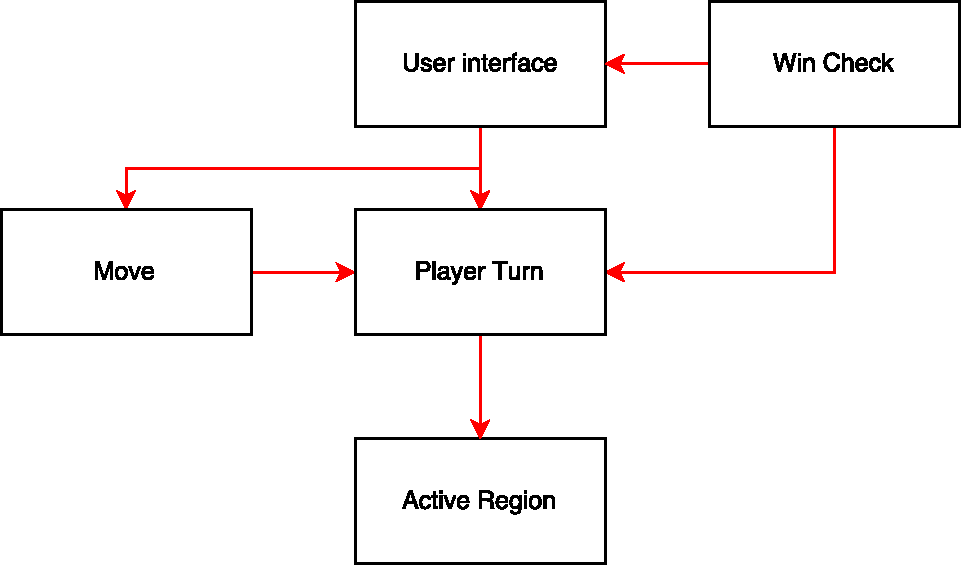
\includegraphics[width=1\textwidth]{UseHierarchy_Diagram.pdf}
\caption{Use hierarchy among modules}
\label{FigUH}
\end{figure}
%\cm{PDF wasn't included in any commits. I don't really like it though. I don't see how the Win Check Model uses the UI. Perhaps more detail on the structure or rework it. I also threw in a sample module hierarchy so that the TeX compiles} \\

\bibliographystyle {plainnat}
\bibliography {MG}


\end{document}